%
% teil1.tex -- Beispiel-File für das Paper
%
% (c) 2020 Prof Dr Andreas Müller, Hochschule Rapperswil
%
% !TEX root = ../../buch.tex
% !TEX encoding = UTF-8
%
\section{Kirchhoffs Gesetz
\label{circuit:section:teil1}}
\rhead{Problemstellung}
Bevor wir die Laplace-Gleichung mithilfe der Lagrange-Funktion herleiten, versuchen wir das auf konventionelle Weise, indem wir  das kirchhoffsche Gesetz benutzen. 
Dafür brauchen wir aber zuerst noch ein paar Erkenntnisse, die hier aufgezeigt werden. Die Stromdichte $\vec{J}$ wird durch
\begin{equation}
	\vec{J}=\frac{\vec{I}}{A}
	\label{circuit:current_density_3}
\end{equation}
definiert. Diese Gleichung besagt, dass die Stromdichte das Verhältnis des Stroms $\vec{I}$ zur Flächen $A$ ist. 
Das kirchhoffsche Stromgesetz postuliert nun, dass die Summe der in einen Knoten einfliessenden Ströme gleich der Summe der aus diesem Knoten ausfliessenden Ströme in einer Schaltung ist. Dies impliziert, dass es in einem Gleichstromkreis im stationären Zustand keine Ladungsakkumulation an irgendeinem Punkt geben kann. Wir betrachten nun einen dreidimensionalen Schaltkreis, in dem die Leitfähigkeit $\sigma$ im gesamten Bereich von Interesse konstant ist. Die Verallgemeinerung des kirchhoffschen Stromgesetzes im dreidimensionalen Fall besagt, dass die Divergenz der Stromdichte $\vec{J}$ gleich Null ist, es kann kein Strom aus dem Nichts erzeugt werden. Daher gilt 
%\eqref{circuit:current_density_1}.
\begin{equation}
	\nabla \cdot  \vec{J}=0.
	\label{circuit:current_density_1}
\end{equation}

Zudem lässt sich der Zusammenhang zwischen dem elektrischen Feld $\vec{E}$ an einem gegebenen Punkt im Raum als negativer Gradient 
\begin{equation}
	\vec{E}=-\nabla \phi
	\label{circuit:current_density_4}
\end{equation}
der Potentialfunktion $\phi$ ausdrücken.

Wenn das elektrische Feld durch $\vec{E}$ repräsentiert wird und wir ein ohmsches Material vorliegen haben, kann die Stromdichte auch als Produkt  
\begin{equation}
\vec{J}=\sigma \vec{E}
\label{circuit:current_density_2}
\end{equation}
beschrieben werden.
Mit dem elektrischen Feld als Gradient von $\phi$ erhalten wir aus der Quellenfreiheit des Stromes \eqref{circuit:current_density_1} und dem ohmschen Gesetz \eqref{circuit:current_density_2} die Differentialgleichung 
\begin{equation}
	\nabla \cdot (\sigma \nabla \phi)=0
	\label{circuit:current_density_5}
\end{equation}
für das Potential $\phi$. Dies kann auch als
\begin{equation}
\nabla^2 \phi=0
\label{circuit:current_density_6}
\end{equation}
geschrieben werden, solange $\sigma$ konstant ist.

\section{Variationsprinzip} 
In diesem Abschnitt wird das Ziel verfolgt, die Gleichung \eqref{circuit:current_density_6} mithilfe eines Variationsprinzips herzuleiten und seine Bedeutung aufzuzeigen. Zunächst werden jedoch die Grundlagen anhand eines einfachen Beispiels wiederholt.
\begin{figure}
	\centering
	\begin{circuitikz}
		\draw (0,3) to[V, v=$U_0$, i=$I_0$] (0,0);
		\draw (0,3) to[short,-*] (3,3)
		to[R, l=$R_1$, i=$I_1$] (3,0) -- (0,0);
		\draw (3,3) -- (6,3)
		to[R, l=$R_2$, i=$I_2$] (6,0) to[short,-*] (3,0);
	\end{circuitikz}
	\caption{Parallelschaltung von $R_1= \SI{2}{\kilo\ohm}$ und $R_2= \SI{1}{\kilo\ohm}$}
	\label{fig:circuit_stromzweig}
\end{figure}

\subsection{Berechnung der Stromverteilung mit klassischen Mitteln} 
Die klassische Methode zur Berechnung der Stromverteilung in einer Parallelschaltung von Widerständen basiert auf dem Ohmschen Gesetz und den Kirchhoffschen Regeln. Das Ohmsche Gesetz lautet:

\begin{equation}
	U=R \cdot I
	\label{circuit:ohmic_law}
\end{equation}

Die Kirchhoffschen Regeln besagen, dass in einem Knotenpunkt eines elektrischen Netzwerkes die Summe der zufliessenden Ströme gleich der Summe der abfliessenden Ströme ist und dass alle Teilspannungen eines Umlaufs bzw. einer Masche in einem elektrischen Netzwerk sich zu null addieren \cite{dewiki:244855415}. Mit diesen Regeln kann man direkt die Ströme in Abbildung \ref{fig:circuit_stromzweig} berechnen und erhält:

\begin{equation}
	I_1 = \frac{I_0 \cdot R_2}{R_1 + R_2} = \frac{\SI{1}{\ampere} \cdot \SI{1}{\kilo\ohm}}{\SI{2}{\kilo\ohm}+ \SI{1}{\kilo\ohm}}=\SI{0.333}{\ampere}
	\label{circuit:current_circuit_power_example3}
\end{equation}

\begin{equation}
	I_2 = I_0-I_1=\SI{1}{\ampere}-\SI{0.333}{\ampere}=\SI{0.667}{\ampere}
	\label{circuit:current_circuit_power4}
\end{equation}
unter der Bedingung das $I_0=\SI{1}{\ampere}$.

Diese Berechnung scheint auf den ersten Blick einfach zu sein, doch es gibt auch eine alternative Methode, das Minimalprinzip, das zum gleichen Ergebnis führt.

\subsection{Das Minimalprinzip als Alternative} 
Das Minimalprinzip bietet eine alternative Methode zur Berechnung der Stromverteilung. Es besagt, dass ein physikalisches System so arbeitet, dass eine bestimmte Größe minimiert wird. In unserem Fall ist diese Größe die Leistung der Schaltung, die durch die Formel
\begin{equation}
	P(I_1)=  I_1^2 \cdot R_1+  (I_0-I_1)^2 \cdot R_2
	\label{circuit:current_circuit_power}
\end{equation}
ausgedrückt wird. Um das Minimum zu finden, leiten wir die Leistung nach $I_1$ ab und setzen die Ableitung gleich Null. Dies führt zu:
\begin{equation}
	\frac{dP}{dI_1} = 2\cdot I_1\cdot R_1 - 2\cdot (I_0 - I_1) \cdot R_2.
	\label{circuit:current_circuit_power1}
\end{equation}
Die zweite Ableitung 
\begin{equation}
	\frac{d^2P}{dI_1^2} = 2\cdot R_1 + 2\cdot R_2
	\label{circuit:current_circuit_power2}
\end{equation}
zeigt eindeutig, dass es sich um ein Minimum handelt, da $R_1$ und $R_2$ positiv sind und daher die zweite Ableitung positiv ist. Wenn wir nun die erste Ableitung \eqref{circuit:current_circuit_power1} gleich Null setzen und auf $I_1$ auflösen bekommen wir
\begin{equation}
	I_1 = \frac{I_0 \cdot R_2}{R_1 + R_2} = \frac{\SI{1}{\ampere} \cdot \SI{1}{\kilo\ohm}}{\SI{2}{\kilo\ohm}+ \SI{1}{\kilo\ohm}}=\SI{0.333}{\ampere}
	\label{circuit:current_circuit_power_a}
\end{equation}
und analog dazu
\begin{equation}
	I_2 = I_0-I_1=\SI{1}{\ampere}-\SI{0.333}{\ampere}=\SI{0.667}{\ampere},
	\label{circuit:current_circuit_power_b}
\end{equation}
wie auch schon in in Gleichung \eqref{circuit:current_circuit_power_example3} und Gelichung \eqref{circuit:current_circuit_power4}.

Dies demonstriert erfolgreich, dass die Verteilung des Stroms in der Schaltung direkt mit der Minimierung der gesamten Leistung korrespondiert. Dies kann auch grafisch wie in Abbildung \ref{fig:circuit_power} dargestellt werden.

\begin{figure}
	\centering
	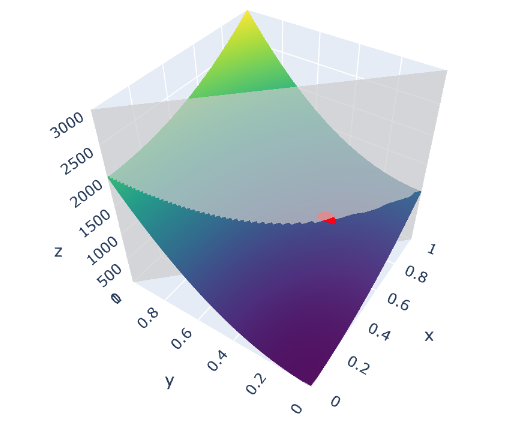
\includegraphics[width=0.7\textwidth]{papers/circuit/two_parrallel_resistors.png}
	\caption{Leistung ($z$-Achse) von zwei parallel geschalteten Widerständen 1 Kilo Ohm ($x$-Achse) und 2 Kilo Ohm ($y$-Achse), in grau dargestellt die Schnittfläche des Stromes von einem Ampere.}
	\label{fig:circuit_power}
\end{figure}

\subsection{Verallgemeinerung auf den stetigen Fall}
Die obige Analyse kann auf den stetigen Fall verallgemeinert werden, indem die Leistung $P$ in einem von einer Oberfläche $S$ umgebenen Volumen $V$ durch 
\begin{equation}
	P=\int_V \sigma(\nabla \phi)^2 d V
	\label{circuit:current_density_7}
\end{equation}
ausdrücken. Wenn wir nun die Euler-Ostrogradski-Differentialgleichung für \eqref{circuit:current_density_7} bestimmen und lösen, gibt uns dies anschliessend die Lösung für die minimale Leistung in einem zweidimensionalen oder dreidimensionalen Raum. D. h. um das Minimum zu finden muss das Integral von \eqref{circuit:current_density_7} minimiert werden. Auf den ersten Blick mag \eqref{circuit:current_density_7} nicht sehr intuitiv erscheinen. Daher könnten wir die Gleichung auch anders formulieren, wie in 
\begin{equation}
	P=\frac{U^2}{R}
	\label{circuit:current_density_8}
\end{equation}
gezeigt, wobei $U^2=\left( \nabla \phi \right)^2$ und $R=\frac{1}{\sigma}$.





%
%
%
%Analog zu dem oben aufgeführten Beispiel können wir die Leistung $P$ in einem von einer Oberfläche $S$ umgebenen Volumen $V$ durch 
%\begin{equation}
%	P=\int_V \sigma(\nabla \phi)^2 d V
%	\label{circuit:current_density_7}
%\end{equation}
%ausdrücken. Wenn wir nun die Euler-Ostrogradski-Differentialgleichung für \eqref{circuit:current_density_7} bestimmen und lösen gibt uns dies anschliessend die Lösung für die minimale Leistung in einem zweidimensionalen oder dreidimensionalen Raum. D.h. um das Minimum zu finden muss das Integral von \eqref{circuit:current_density_7} minimiert werden. Auf den ersten Blick mag \eqref{circuit:current_density_7} nicht sehr intuitiv erscheinen. Daher könnten wir die Gleichung auch anders formulieren, wie in 
%\begin{equation}
%	P=\frac{U^2}{R}
%	\label{circuit:current_density_8}
%\end{equation}
%gezeigt, wobei $U^2=\left( \nabla \phi \right)^2$ und $R=\frac{1}{\sigma}$.


\section{Herleitung der Laplace-Gleichung}
In diesem Kapitel leiten wir die Laplace-Gleichung her. Die Herleitung basiert auf der Euler-Ostrogradski-Differentialgleichung, die in Gleichung \eqref{buch:felder:ostrogradski:eqn:euler-ostrogradski} dargestellt ist.

Wir beginnen mit Gleichung \eqref{circuit:current_density_7} und wenden darauf die genannte Differentialgleichung an:
\begin{enumerate}
	\item Schritt: Lagrange-Funktion des Problems ohne $\sigma$ (da wir das Minimum suchen und $\sigma$ eine Konstante ist hat $\sigma$ keinen Einfluss auf die Lösung und kann daher weggelassen werden)
	\begin{equation}
		L(U, U_x)= U_x^2 = (U_{x_1}^2+U_{x_2}^2).
	\end{equation}
	\item Schritt: partielle Ableitungen
	\begin{equation}
		\begin{aligned}
			\frac{\partial L}{\partial U}&=0\\
			\frac{\partial L}{\partial U_{x_1}}&=2U_{x_1}\\
			\frac{\partial L}{\partial U_{x_2}}&=2U_{x_2}.\\
		\end{aligned}
	\end{equation}
	\item Schritt: Ableiten nach $x_1$ und $x_2$
	\begin{equation}
		\begin{aligned}
			\frac{\partial}{\partial x_1}\frac{\partial L}{\partial U_{x_1}}(x,\phi,\nabla \phi)=2\frac{\partial \phi}{\partial {x_1}}\cdot \frac{\partial}{\partial x_1},\\
			\frac{\partial}{\partial x_2}\frac{\partial L}{\partial U_{x_2}}(x,\phi,\nabla \phi)=2\frac{\partial \phi}{\partial {x_2}} \cdot \frac{\partial}{\partial x_1}.\\
		\end{aligned}
	\end{equation}
	\item Schritt: Euler-Ostrogradski Differentialgleichung
	\begin{equation}
		0=-\frac{\partial}{\partial x_1}\cdot 2\frac{\partial \phi}{\partial {x_1}}-\frac{\partial}{\partial x_2}\cdot 2\frac{\partial \phi}{\partial {x_2}}=-2\Delta\phi.
	\end{equation}
\end{enumerate}

Das Ergebnis der Anwendung der Theorie der Euler-Ostrogradski-Differentialgleichung ist:
	\begin{equation}
	\sigma \cdot 2\Delta\phi=0.
	\end{equation}
Wir können nun noch durch $2\sigma$ teilen und erhalten die Laplace-Gleichung aus \eqref{circuit:current_density_6}. Somit wurde gezeigt, dass die Laplace-Gleichung sowohl durch das Variationsprinzip als auch durch die Kirchhoffschen Regeln gefunden werden kann.



\section{Praktische Anwendungen}
In diesem Abschnitt werden wir die numerische Lösung der elliptischen partiellen Differentialgleichung \eqref{circuit:current_density_6} untersuchen und ihre Bedeutung erläutern.

\subsection{Diskretisierung der Ableitungen} Die Gleichung \eqref{circuit:current_density_6} kann durch eine Differenz zweiter Ordnung diskretisiert werden, wie in Gleichung \eqref{circuit:second-order-central} dargestellt:

\begin{equation}
	f^{\prime \prime}(x) \approx \frac{\delta_h^2[f](x)}{h^2}=\frac{\frac{f(x+h)-f(x)}{h}-\frac{f(x)-f(x-h)}{h}}{h}=\frac{f(x+h)-2 f(x)+f(x-h)}{h^2}.
	\label{circuit:second-order-central}
\end{equation}
\cite{enwiki:1220817436}

\subsection{Diskretisierung in zwei Dimensionen} Um diese Diskretisierung auf unseren zweidimensionalen Fall anzuwenden, führen wir ein Gitter ein, dessen Punkte durch die Koordinaten $(x_i, y_j)$ repräsentiert werden. Die Differenzen zwischen den Gitterpunkten in x- und y-Richtung werden durch $\Delta x$ und $\Delta y$ dargestellt. Dies führt zu folgender diskretisierter Gleichung:
\begin{equation}
	\frac{\phi(x_{i+1}, y_j) - 2\phi(x_i, y_j) + \phi(x_{i-1}, y_j)}{(\Delta x)^2} + \frac{\phi(x_i, y_{j+1}) - 2\phi(x_i, y_j) + \phi(x_i, y_{j-1})}{(\Delta y)^2} = 0.
	\label{circuit:discret_equation}
\end{equation}

\subsection{Auflösen nach $\phi(x_i, y_j)$} 
Wir können nun nach $\phi(x_i, y_j)$ auflösen und erhalten:
\begin{equation}
	\phi(x_i, y_j) = \frac{1}{4}(\phi(x_{i+1}, y_{j}) + \phi(x_{i-1}, y_{j}) + \phi(x_{i}, y_{j+1}) + \phi(x_{i}, y_{j-1})).
	\label{circuit:discret_equation2}
\end{equation}
Diese Gleichung ermöglicht es uns, das Potential an jedem Gitterpunkt zu berechnen, indem wir die Potentiale der umliegenden Punkte verwenden. Die Form von \eqref{circuit:discret_equation2} ist eine andere Darstellung von \eqref{circuit:discret_equation} für die numerische Implementierung.

\subsection{Numerisches Beispiel} 
\subsubsection{Quadratisches Kontakt}
Betrachten wir als Beispiel eine leitende Platte mit einer Leitfähigkeit von \SI{0.001}{\siemens\per\meter} und einer Größe von einem Quadratmeter. Ein spezifischer Bereich der Platte, Quadrat definiert durch $0.5 < x < 0.7$ und $0.5 < y < 0.7$, wird mit einem Potential von einem Volt belegt, während der Rand der Platte ein Potential von 0 Volt aufweist.

\begin{figure}
	\centering
	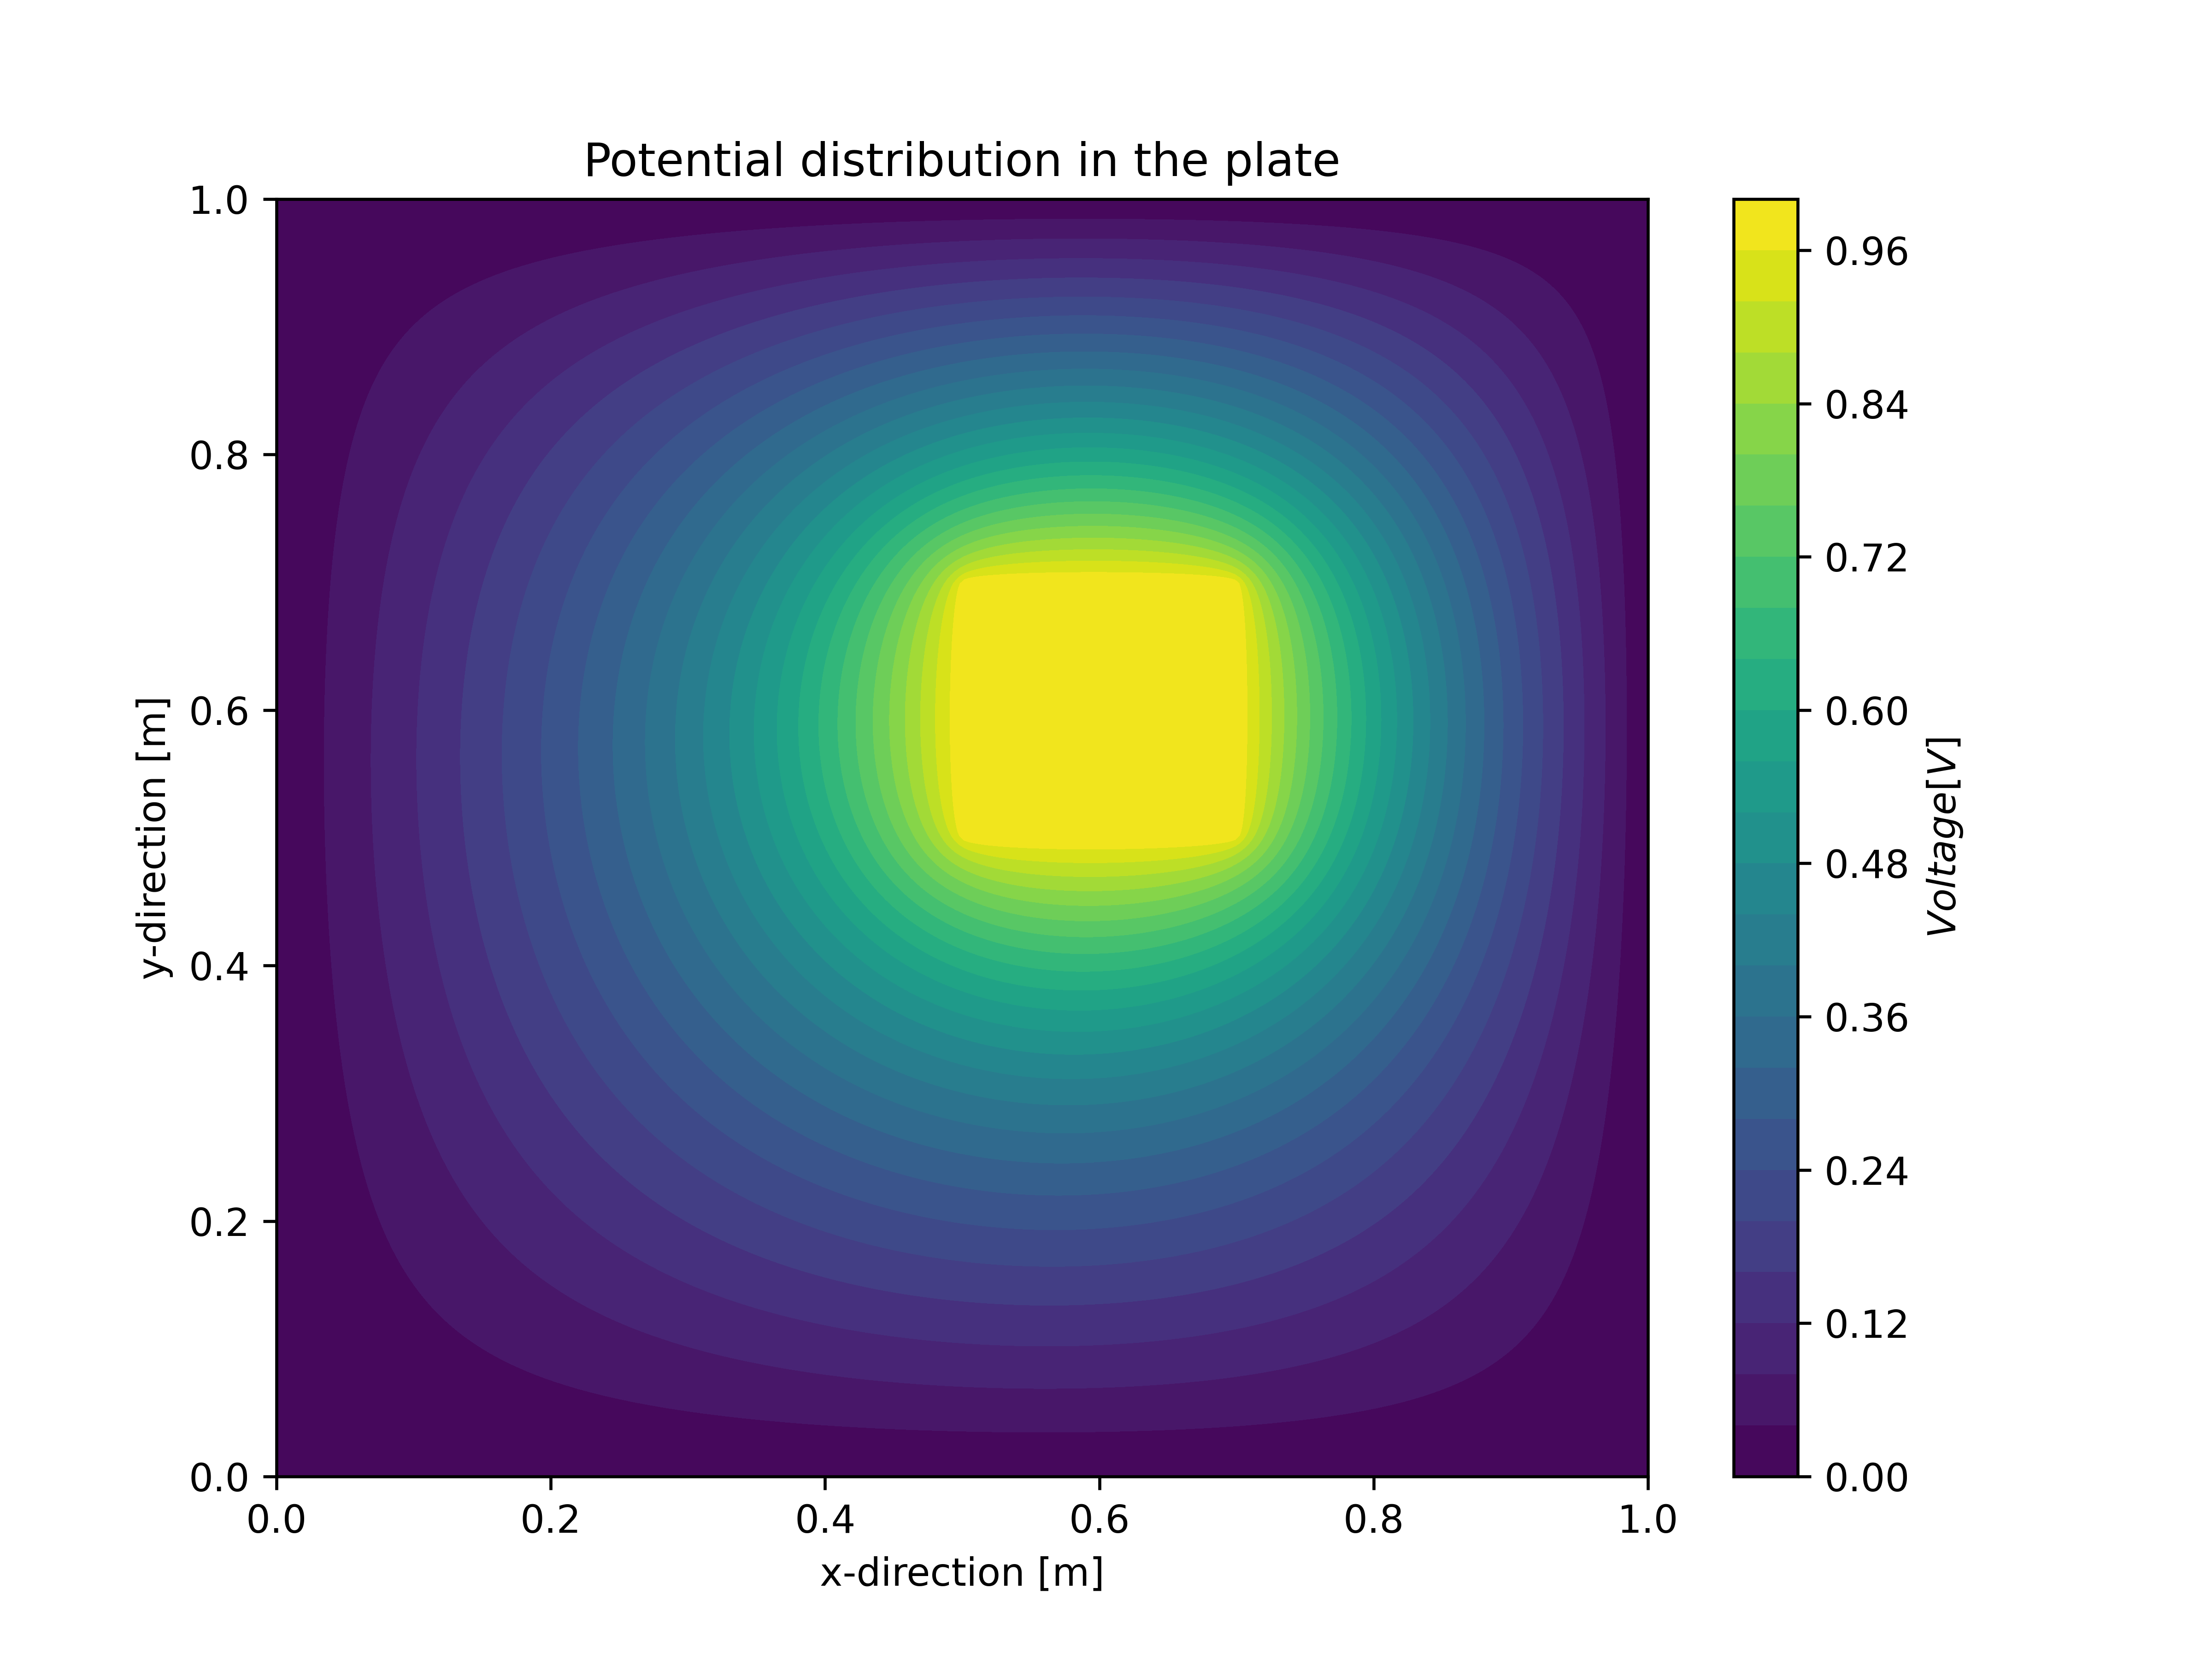
\includegraphics[width=0.99\textwidth]{papers/circuit/potential_distribution.png}
	\caption{Potential-Verteilung auf rechteckiger Platte mit rechteckigem Potential im oberen rechten Bereich und 0 Potential am Rand der Platte \cite{github:AndreasFMueller}}
	\label{fig:potential_distribution}
\end{figure}
Unter Verwendung von Gleichung \eqref{circuit:discret_equation2} zur Berechnung des Potentials und den gegebenen Randbedingungen erhalten wir die in Abbildung \ref{fig:potential_distribution} dargestellte Potentialverteilung. Dies ermöglicht uns, das gesamte Potential auf der Platte zu bestimmen.

Sobald das Potential bekannt ist, können wir mithilfe des Gradienten und Gleichung \eqref{circuit:current_density_7} die Leistungsdichte an jedem einzelnen Punkt berechnen. Dies führt zu den in Abbildung \ref{fig:power_2d} und \ref{fig:power_3d_rectangle} dargestellten Leistungsdichteverteilung.
\begin{figure}[h]
	\centering
	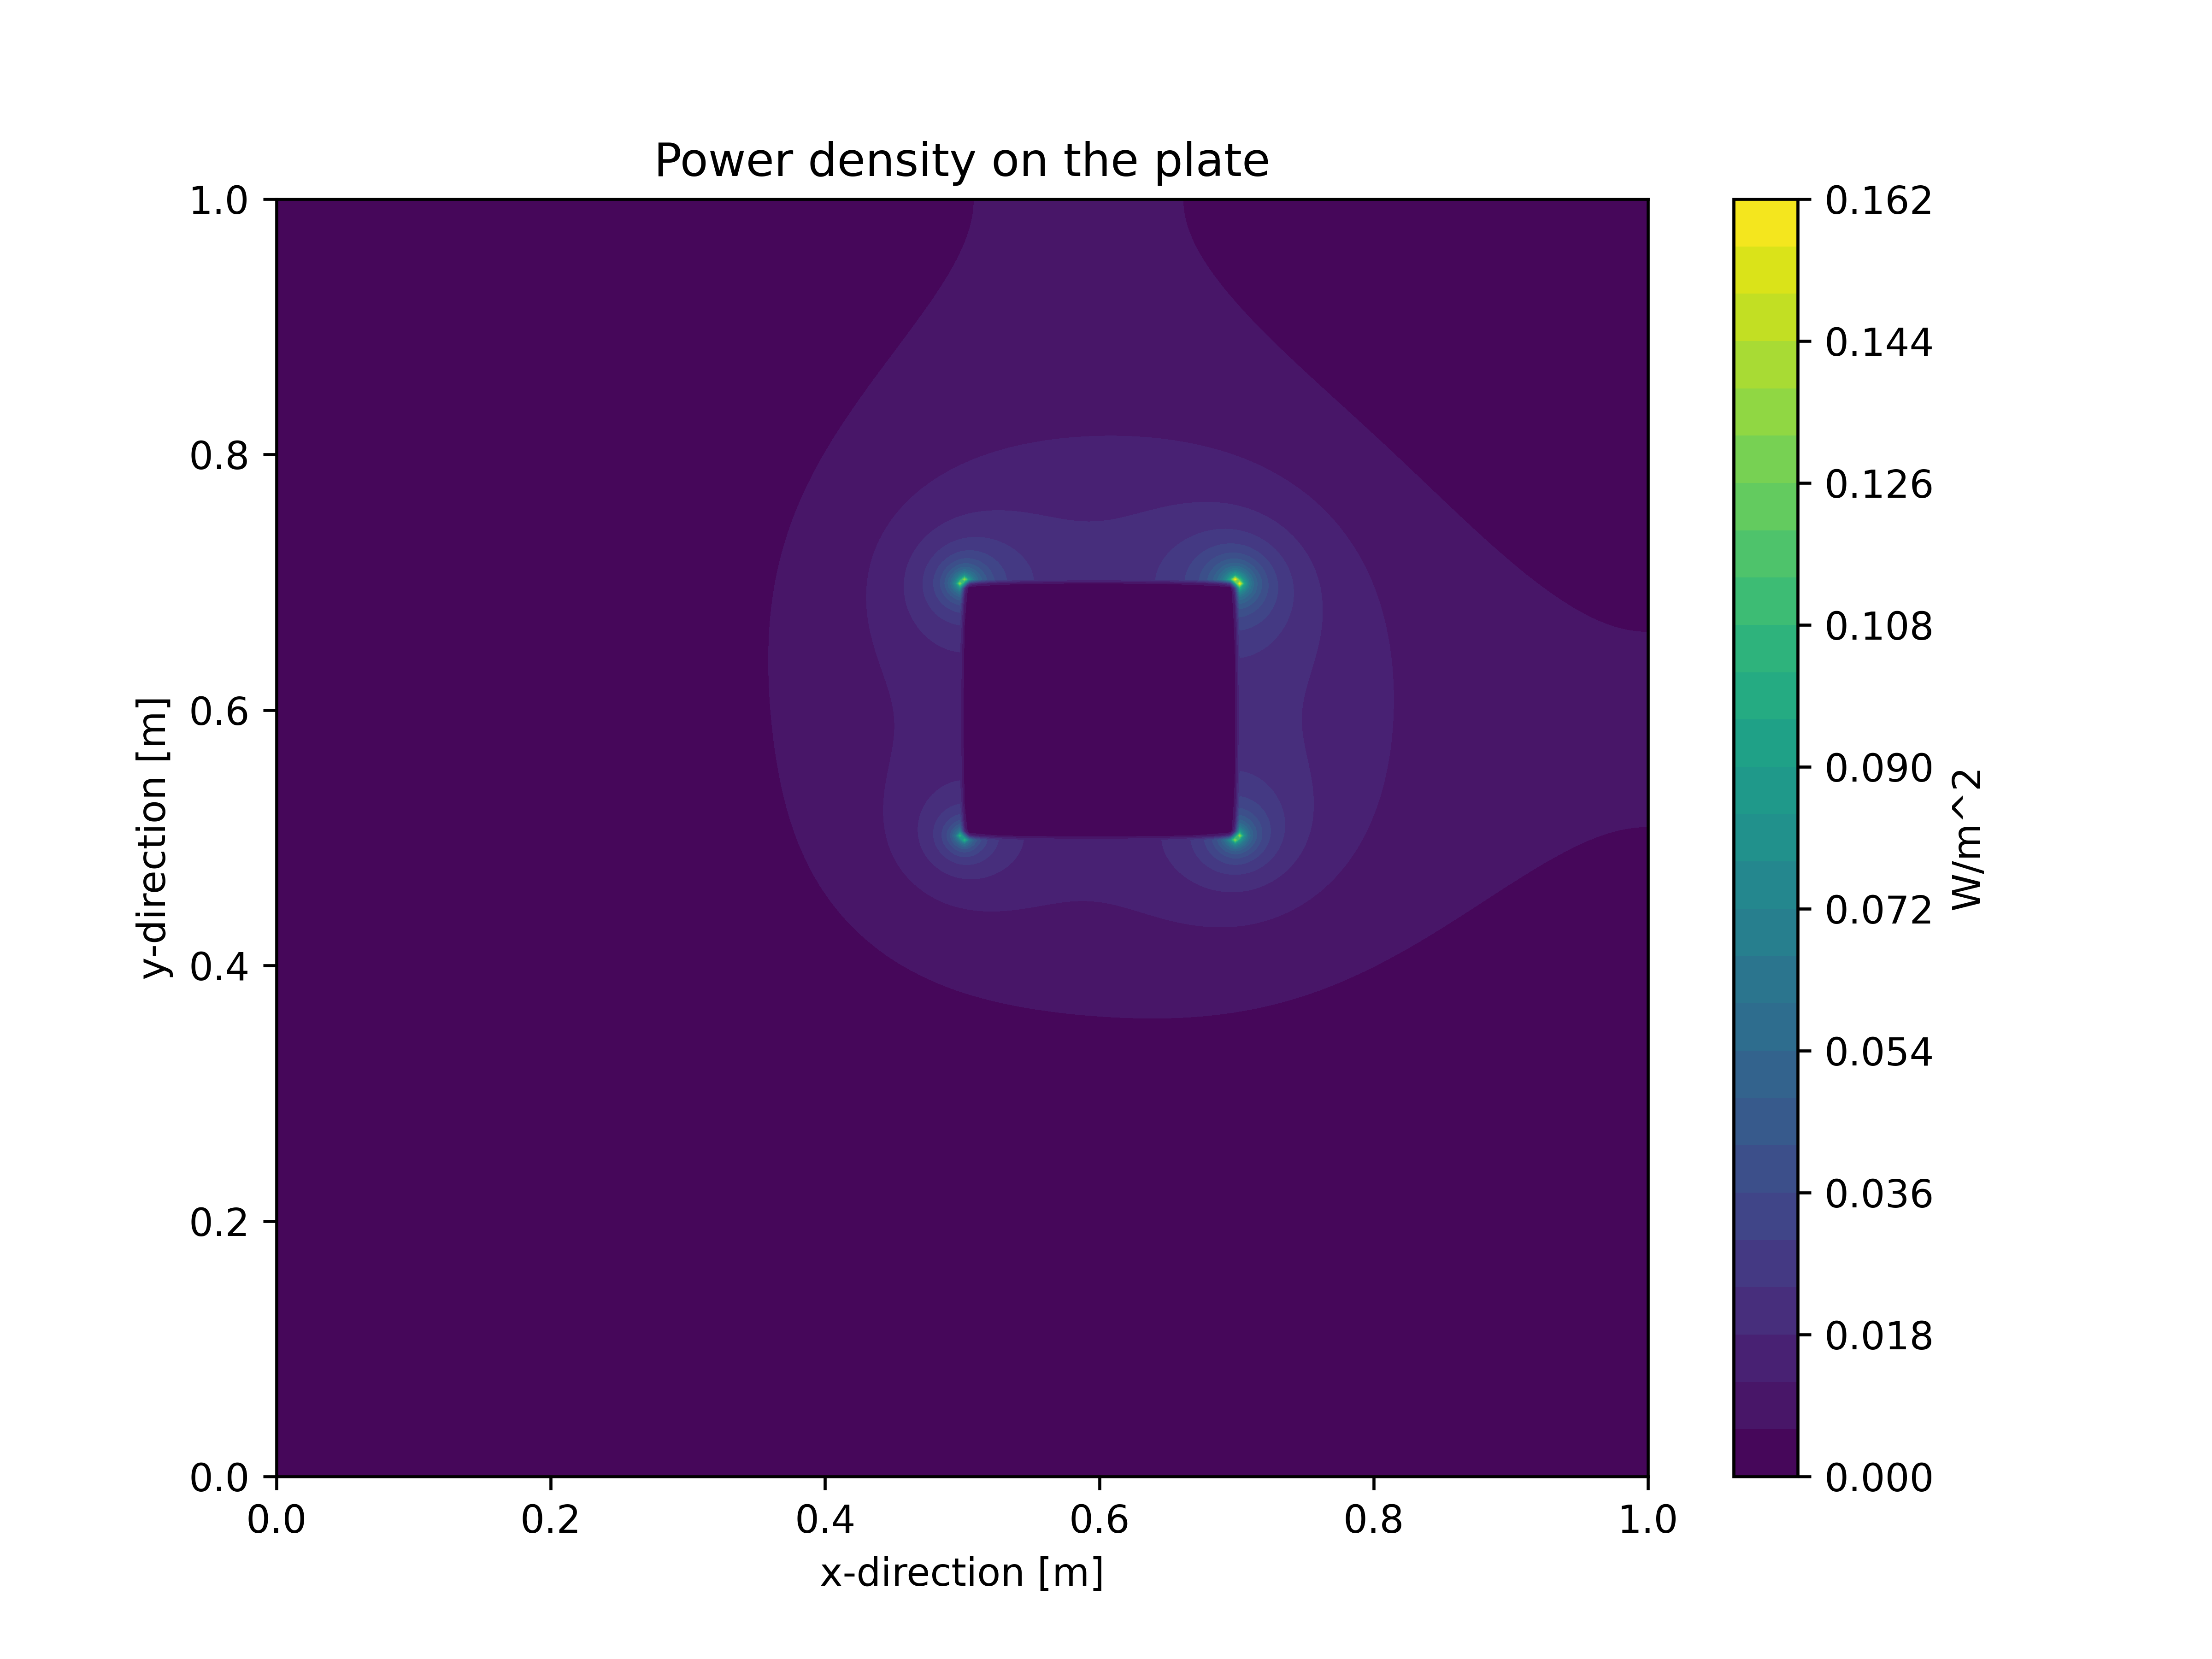
\includegraphics[width=0.99\textwidth]{papers/circuit/power_distribution.png}
	\caption{Leistungsdichte auf rechteckiger Platte mit rechteckigem Potential im oberen rechten Bereich und 0 Potential am Rand der Platte. (Code für die Generierung des Plots kann in \cite{github:AndreasFMueller} gefunden werden.)}
	\label{fig:power_2d}
\end{figure}
\begin{figure}[h]
	\centering
	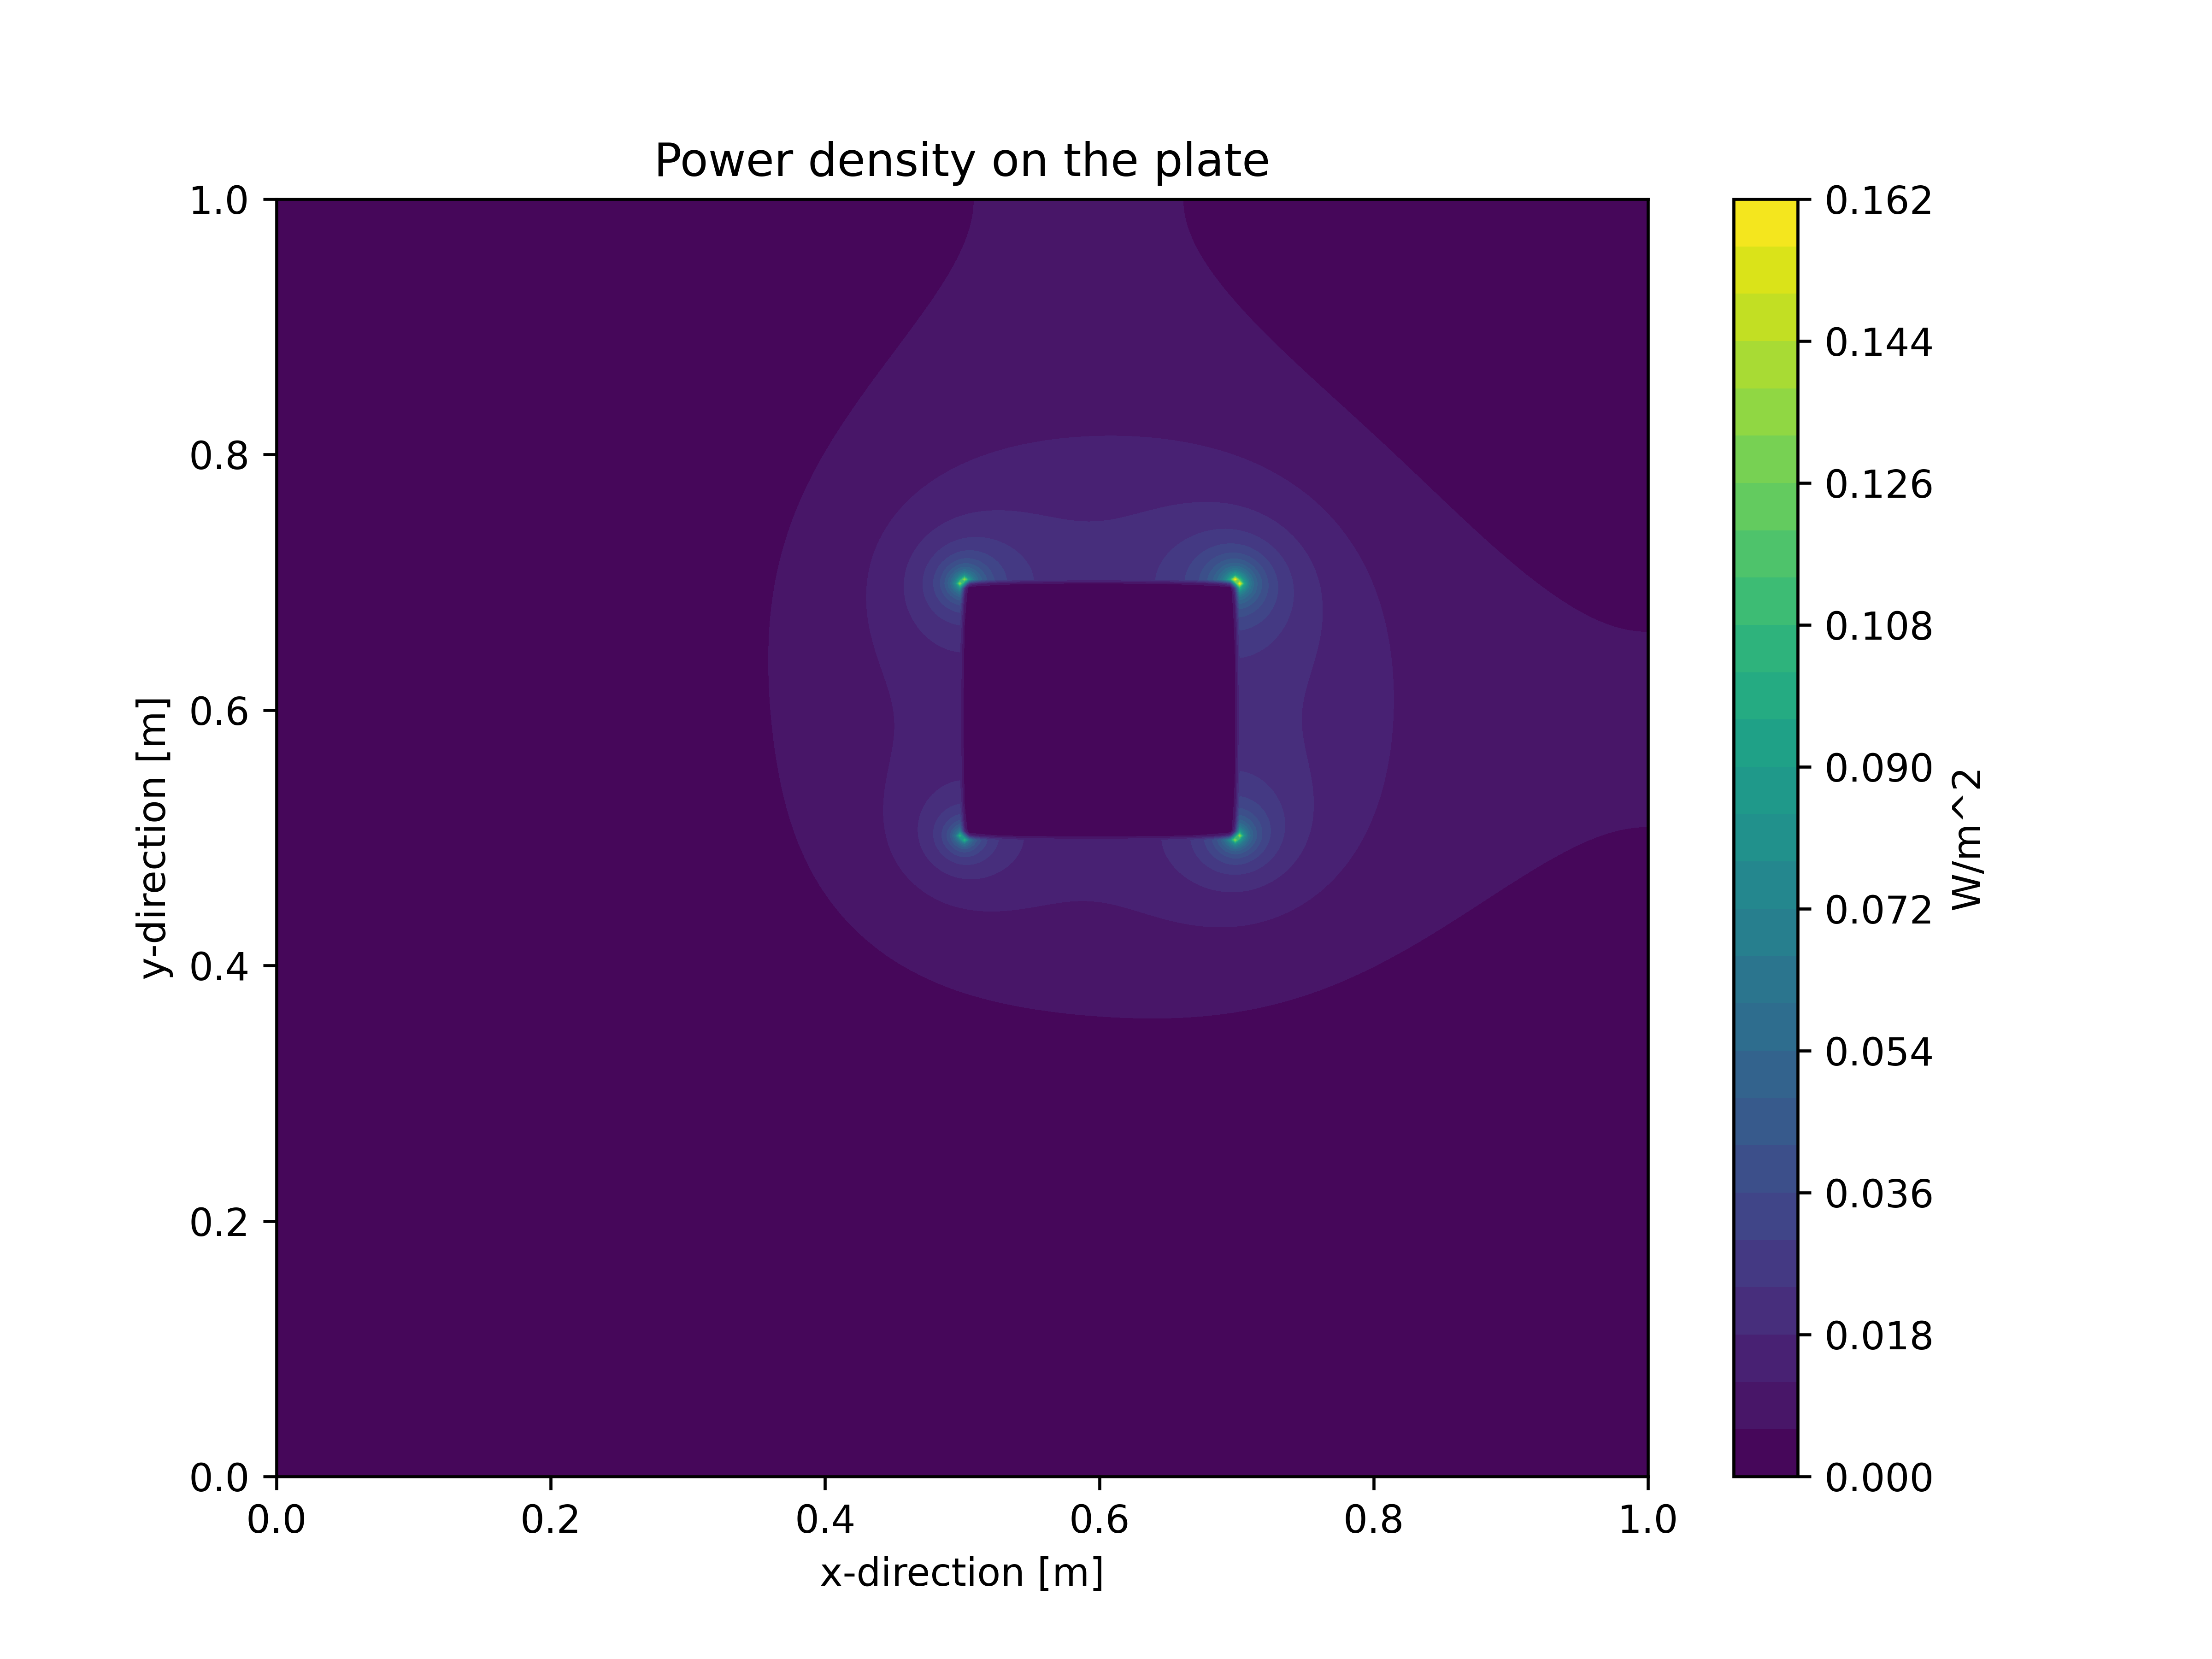
\includegraphics[width=0.99\textwidth]{papers/circuit/power_distribution_circle.png}
	\caption{Leistungsdichte auf rechteckiger Platte mit kreisförmigen Potential im oberen rechten Bereich und 0 Potential am Rand der Platte. (Code für die Generierung des Plots kann in \cite{github:AndreasFMueller} gefunden werden.)}
	\label{fig:power_2d_circle}
\end{figure}
\begin{figure}[h]
	\centering
	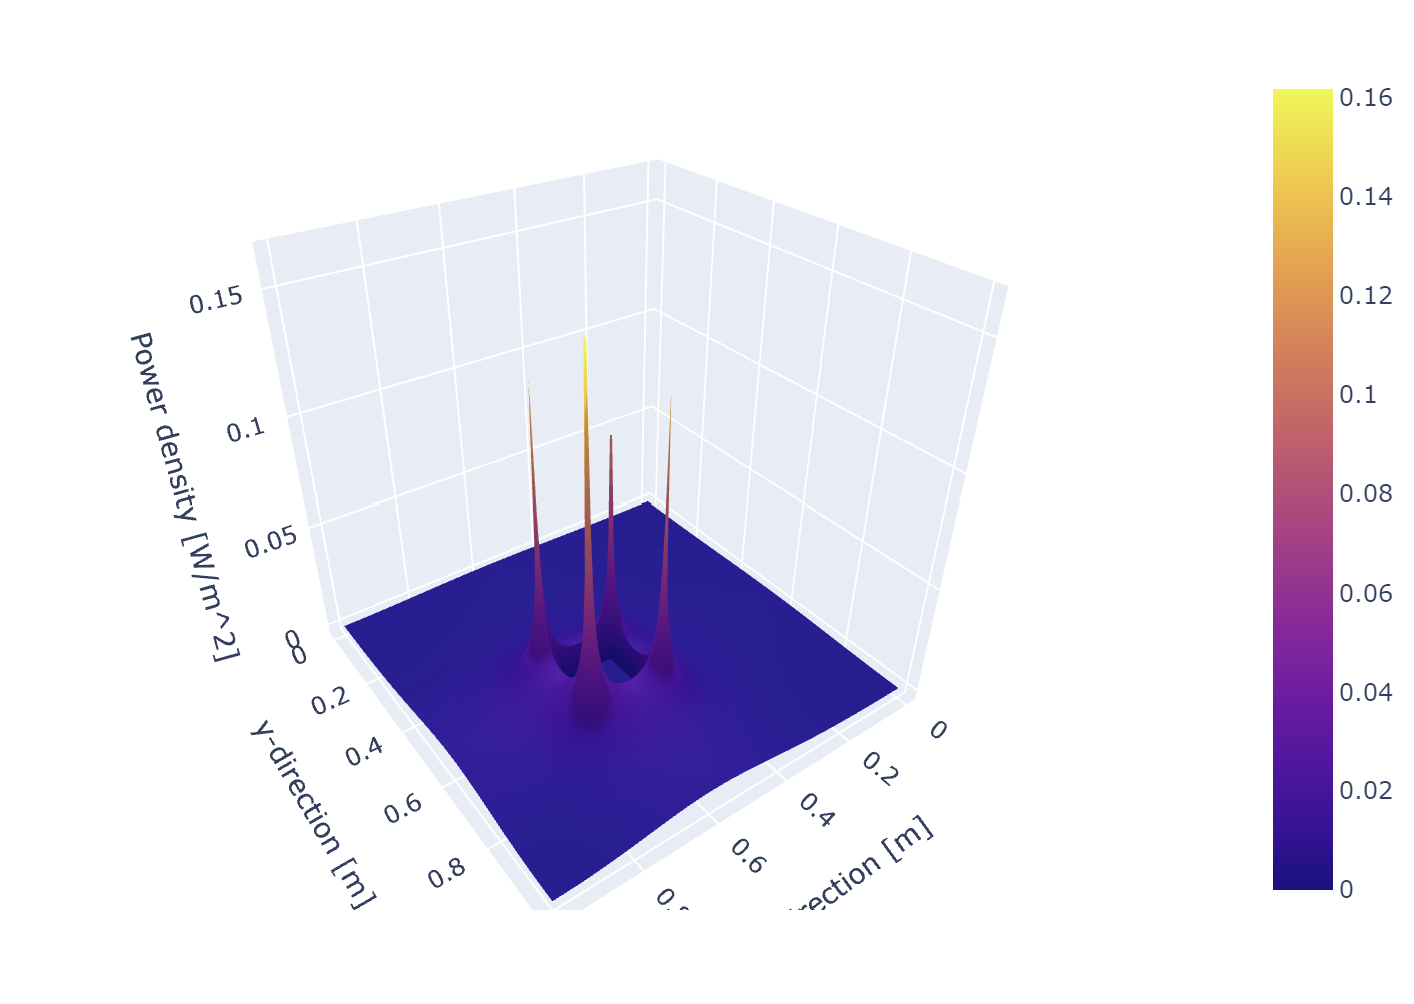
\includegraphics[width=0.99\textwidth]{papers/circuit/3d.png}
	\caption{Leistungsdichte 3d auf rechteckiger Platte mit rechteckigem Potential und 0 Potential am Rand der Platte. (Code für die Generierung des Plots kann in \cite{github:AndreasFMueller} gefunden werden.)}
	\label{fig:power_3d_rectangle}
\end{figure}
\begin{figure}[h]
	\centering
	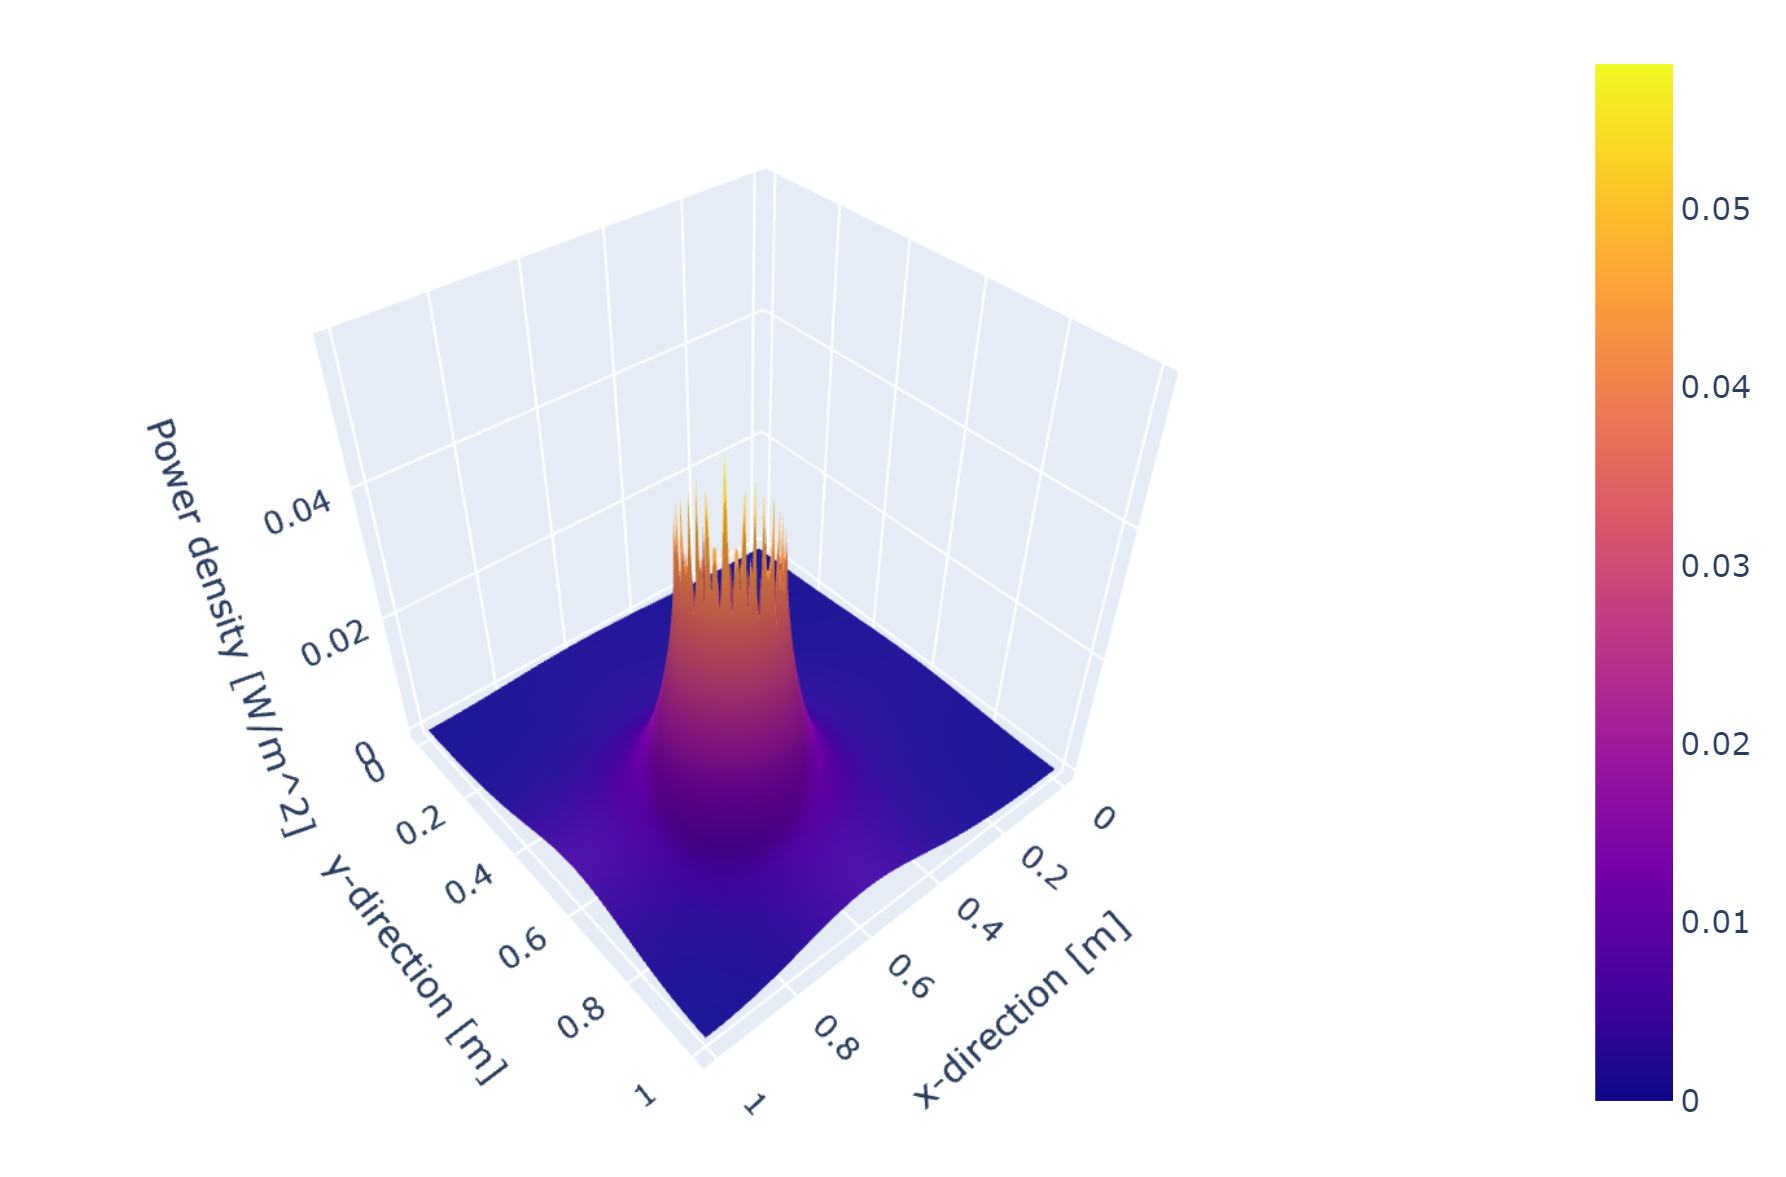
\includegraphics[width=0.99\textwidth]{papers/circuit/3d_circle.png}
	\caption{Leistungsdichte 3d auf rechteckiger Platte mit kreisförmigen Potential und 0 Potential am Rand der Platte. (Code für die Generierung des Plots kann in \cite{github:AndreasFMueller} gefunden werden.)}
	\label{fig:power_3d_circle}
\end{figure}
Abbildung \ref{fig:power_3d_rectangle} zeigt deutlich, dass die Leistungsdichte in den Ecken des zuvor definierten quadratischen Potentials am höchsten ist. Dies ist unter anderem ein Grund, warum auf Leiterplatten normalerweise keine 90°-Winkel für Leiterbahnen gezeichnet werden, sondern meistens 45°-Winkel verwendet werden, um die Leistungsdichte bzw. Stromdichte in den Ecken zu minimieren.

\subsubsection{Kreisförmiges Kontakt} Wenn wir anstelle eines rechteckigen Potentials ein kreisförmiges Potential verwenden, ist die Leistungsdichte deutlich geringer, wie in Abbildung \ref{fig:power_3d_circle} und Abbildung \ref{fig:power_2d_circle} dargestellt. Daher ist es vorteilhaft, abgerundete Ecken zu verwenden, wenn man die Leistungsdichte auf einer Leiterbahn minimieren möchte.

Diese Beispiele illustrieren die praktische Anwendung des Variationsprinzips und der numerischen Lösung von partiellen Differentialgleichungen in der Elektrotechnik. Sie zeigen, wie die Form von Leiterbahnen auf einer Leiterplatte optimiert werden können, um die Leistungsdichte zu minimieren und die Effizienz zu maximieren.